%---------------------------------------------------
% Pesquisa Bibliográfica
%---------------------------------------------------

\localtableofcontents*


Para o desenvolvimento deste trabalho, reconhecimento de acordes naturais de guitarra utilizando redes neurais artificiais, é necessário abordar alguns conceitos fundamentais e indispensáveis à sua construção, como apresentado a seguir.

\section{Formação de Acordes}

Em sua estrutura, a música possui características que podem ser descritas e analisadas através da transforma discreta de Fourier (\textit{Discret Transform Fourier})\footnote{Jean Baptiste Joseph Fourier (1768 - 1830) - Matemático e Físico Francês. Em 1807 terminou um de seus trabalhos onde observou que séries senoidais harmonicamente relacionadas eram úteis na representação da distribuição de temperatura em um corpo. Afirmou ainda que 'qualquer' sinal periódico poderia ser representado por tal série, que leva o seu nome em sua homenagem \cite{oppen2010}.}, num dos tópicos que será tratado a seguir. A relação entre as notas que compõem um acorde são semelhantes à análise feita pelas técnicas Fourier.



\subsection{Definições}

Para tratar de formação de acordes é necessário comentar sobre algumas definições relevantes, a saber:

\begin{itemize}
   \item Altura - é a propriedade que nos permite diferenciar os sons mais graves dos mais agudos, guardando uma relação direta com a frequência de vibração da onda sonora. Quanto maior for a frequência, mais agudo será o som, analogamente, sons mais graves estão associados a baixas frequências de oscilações \cite{med1996}; 
   \item Intensidade - Refere-se a amplitude de um sinal, indicando se um som é forte ou fraco;
   \item Duração - Tempo de reprodução de um som;
   \item Timbre - é a qualidade pela qual podemos diferenciar dois sons musicais produzidos por fontes sonoras diferentes, ainda que possuam a mesma altura e intensidade. É através do timbre que conseguimos distinguir claramente a diferença entre instrumentos, ou vozes humanas, que estão emitindo uma mesma nota \cite{moyses2002};  
   \item Nota - Nomenclatura dada a representação de um som (frequência) na música. Sendo essas, representadas pelas letras, C (Dó), D (Ré), E (Mi), F (Fá), G (Sol), A (Lá) e B (Si) no inglês; pois, no alemão a nota B representa "si bemol", enquanto o H (Si) \cite{med1996};
   \item Acorde - Combinação de três ou mais sons (notas) simultâneos \cite{med1996}. Em frequência, esses sons referem-se a três ou mais frequências simultâneas;
%   \item Sistema Natural - A escala natural é a escala conhecida como Pitagórica
   \item Sistema Temperado - A definição abordada em \citeonline{med1996} é de que no sistema temperado os semitons (intervalo entre duas notas consecutivas) são perfeitamente iguais, ficando cada semitom com quatro comas\footnote{do grego \textit{koma}, a nona parte de um tom, \cite[p. 31]{med1996}.} e meia;%. Representa o abandono da perfeição da afinação absoluta no sistema natural, facilitando as projeções cromáticas;
   \item Intervalo - É a diferença de altura entre dois sons  (notas). O mesmo é denominado de acordo com o número de notas que o compreendem \cite{med1996};
   \item Semitom(ST) - É o menor intervalo e entre duas notas consecutivas na música ocidental (sistema temperado) \cite{med1996};
   \item Tom (T) - Intervalo composto por dois semitons (ST);
   \item Escalas - Conjunto de notas encadeadas numa lei de formação, intervalos específicos, para cada tipo de escala. Nesse trabalho o foco está na escala natural ou diatônica, 7 notas numa oitava\footnote{Conjunto de notas existentes entre uma nota e sua primeira repetição no agudo ou no grave \cite{lacerda1967}. Em frequência, o dobro ou metade da frequência respectivamente.};
   \item Escala\footnote{do latim \textit{scala}, que significa gama ou escada.\cite{med1996}.} Temperada - Consiste na divisão da escala em doze semitons iguais. Dessa forma para um instrumento temperado, um semitom equivale a $\sqrt[12]{2}\approx1,0595$ Hz, ou seja qualquer valor de frequência que se deseje encontrar seguirá a relação $f_{k+1} = f_k\times2^{1/12}$;
   \item Série Harmônica - conjunto de sons que acompanham um som fundamental. Toda nota gera uma série harmônica proporcionalmente idêntica \cite[p. 92]{med1996}.
\end{itemize}

%% ************************************
\subsection{Escalas Maior e Menor}
%% ************************************

Seguindo essa definição, na \autoref{tab:acordes} são apresentados os acordes que deverão ser reconhecidos pelo sistema.

\newcolumntype{g}{>{\columncolor{lightgray}}c}  % Comando para colorir colunas
\begin{table}[H]
   \caption{Mapa dos acordes maiores e menores a serem reconhecidos.}
   \label{tab:acordes}
   \begin{threeparttable}
   \begin{tiny}
   \centering
   \resizebox{\linewidth}{!}{% Resize table to fit within \linewidth horizontally
   \setlength{\extrarowheight}{3pt}       %%Aumentar a altura das linhas
   \begin{tabular}{cgcgcgcgcgcgc}\hline
   \multicolumn{13}{c}{Mapa de Acordes Naturais} \\
   \toprule
Maiores                & C        & C\#    & D   & D\#    & E   & F   & F\#    & G   & G\#      & A   & A\#   & B   \\ \midrule
\multirow{3}{*}{Notas} & C        & C\#    & D   & D\#    & E   & F   & F\#    & G   & G\#      & A   & A\#   & B   \\
                       & E        & F      & F\# & G      & G\# & A   & A\#    & B   & C        & C\# & D     & D\# \\
                       & G        & G\#    & A   & A\#    & B   & C   & C\#    & D   & D\#      & E   & F     & F\# \\ \midrule
Menores                & Cm       & C\#{m} & Dm  & D\#{m} & Em  & Fm  & F\#{m} & Gm  & G\#{m}   & Am  & A\#{m}& Bm  \\ \midrule
\multirow{3}{*}{Notas} & C        & C\#    & D   & D\#    & E   & F   & F\#    & G   & G\#      & A   & A\#   & B   \\ 
                       & E$\flat$ & E      & F   & F\#    & G   & G\# & A      & A\# & B$\flat$ & C   & C\#   & D   \\
                       & G        & G\#    & A   & A\#    & B   & C   & C\#    & D   & D\#      & E   & F     & F\# \\ \bottomrule                     
   \end{tabular}}
   \end{tiny}
   \end{threeparttable}
   %\legend{Fonte: o autor}
\end{table}%
Para o desenvolvimento deste trabalho, reconhecimento de acordes naturais de guitarra utilizando redes neurais artificiais, é necessário abordar alguns conceitos fundamentais e indispensáveis à sua construção, como apresentado a seguir.

\section{Formação de Acordes}

Em sua estrutura, a música possui características que podem ser descritas e analisadas através da transforma discreta de Fourier (\textit{Discret Transform Fourier})\footnote{Jean Baptiste Joseph Fourier (1768 - 1830) - Matemático e Físico Francês. Em 1807 terminou um de seus trabalhos onde observou que séries senoidais harmonicamente relacionadas eram úteis na representação da distribuição de temperatura em um corpo. Afirmou ainda que 'qualquer' sinal periódico poderia ser representado por tal série, que leva o seu nome em sua homenagem \cite{oppen2010}.}, num dos tópicos que será tratado a seguir. A relação entre as notas que compõem um acorde são semelhantes à análise feita pelas técnicas Fourier.

%% SIMAS
%Em sua estrutura, a música possui uma relação muito próxima com a série de Fourier \footnote{Jean Baptiste Joseph Fourier (1768 - 1830) - Matemático e Físico Francês. Em 1807 terminou um de seus trabalhos onde observou que séries senoidais harmonicamente relacionadas eram úteis na representação da distribuição de temperatura em um corpo. Afirmou ainda que 'qualquer' sinal periódico poderia ser representado por tal série, que leva o seu nome em sua homenagem \cite{oppen2010}.}, um dos tópicos que será tratado a seguir. Relação essa que pode ser tomada como exemplo direto, no caso dos acordes, pois, cada acorde é formado por um conjunto de notas, e na abordagem desse documento, o foco estará nas frequências que o compõem.


\subsection{Definições}

Para tratar de formação de acordes é necessário comentar sobre algumas definições relevantes, a saber:

\begin{itemize}
   \item Altura - é a propriedade que nos permite diferenciar os sons mais graves dos mais agudos, guardando uma relação direta com a frequência de vibração da onda sonora. Quanto maior for a frequência, mais agudo será o som, analogamente, sons mais graves estão associados a baixas frequências de oscilações \cite{med1996}; 
   \item Intensidade - Refere-se a amplitude de um sinal, indicando se um som é forte ou fraco;
   \item Duração - Tempo de reprodução de um som;
   \item Timbre - é a qualidade pela qual podemos diferenciar dois sons musicais produzidos por fontes sonoras diferentes, ainda que possuam a mesma altura e intensidade. É através do timbre que conseguimos distinguir claramente a diferença entre instrumentos, ou vozes humanas, que estão emitindo uma mesma nota \cite{moyses2002};  
   \item Nota - Nomenclatura dada a representação de um som (frequência) na música. Sendo essas, representadas pelas letras, C (Dó), D (Ré), E (Mi), F (Fá), G (Sol), A (Lá) e B (Si) no inglês; pois, no alemão a nota B representa "si bemol", enquanto o H (Si) \cite{med1996};
   \item Acorde - Combinação de três ou mais sons (notas) simultâneos \cite{med1996}. Em frequência, esses sons referem-se a três ou mais frequências simultâneas;
%   \item Sistema Natural - A escala natural é a escala conhecida como Pitagórica
   \item Sistema Temperado - A definição abordada em \citeonline{med1996} é de que no sistema temperado os semitons (intervalo entre duas notas consecutivas) são perfeitamente iguais, ficando cada semitom com quatro comas\footnote{do grego \textit{koma}, a nona parte de um tom, \cite[p. 31]{med1996}.} e meia;%. Representa o abandono da perfeição da afinação absoluta no sistema natural, facilitando as projeções cromáticas;
   \item Intervalo - É a diferença de altura entre dois sons  (notas). O mesmo é denominado de acordo com o número de notas que o compreendem \cite{med1996};
   \item Semitom(ST) - É o menor intervalo e entre duas notas consecutivas na música ocidental (sistema temperado) \cite{med1996};
   \item Tom (T) - Intervalo composto por dois semitons (ST);
   \item Escalas - Conjunto de notas encadeadas numa lei de formação, intervalos específicos, para cada tipo de escala. Nesse trabalho o foco está na escala natural ou diatônica, 7 notas numa oitava\footnote{Conjunto de notas existentes entre uma nota e sua primeira repetição no agudo ou no grave \cite{lacerda1967}. Em frequência, o dobro ou metade da frequência respectivamente.};
   \item Escala\footnote{do latim \textit{scala}, que significa gama ou escada.\cite{med1996}.} Temperada - Consiste na divisão da escala em doze semitons iguais. Dessa forma para um instrumento temperado, um semitom equivale a $\sqrt[12]{2}\approx1,0595$ Hz, ou seja qualquer valor de frequência que se deseje encontrar seguirá a relação $f_{k+1} = f_k\times2^{1/12}$;
   \item Série Harmônica - conjunto de sons que acompanham um som fundamental. Toda nota gera uma série harmônica proporcionalmente idêntica \cite[p. 92]{med1996}.
\end{itemize}

%% ************************************
\subsection{Escalas Maior e Menor}
%% ************************************

Como apresentado anteriormente, a escala natural possui 7 notas. A partir dessa definição existem diversas combinações entre essas 7 notas, com seus respectivos nomes. Nesse trabalho foi proposto a identificação de acordes maiores e menores, das escalas naturais, ou seja escala Maior Natural e Menor Natural.

Numa escala natural, o intervalo compreendido entre a primeira nota e a última contém 6 tons (Ts), ou 12 semitons (STs). 

Escala Maior é uma escala diatônica que possui dois semitons entre o III--IV e VII--I graus, conforme \autoref{fig:escalaMaior} \cite{med1996}.

\begin{figure}[H]
   \begin{center}   
      \caption{Escala Maior.}
      \label{fig:escalaMaior}
      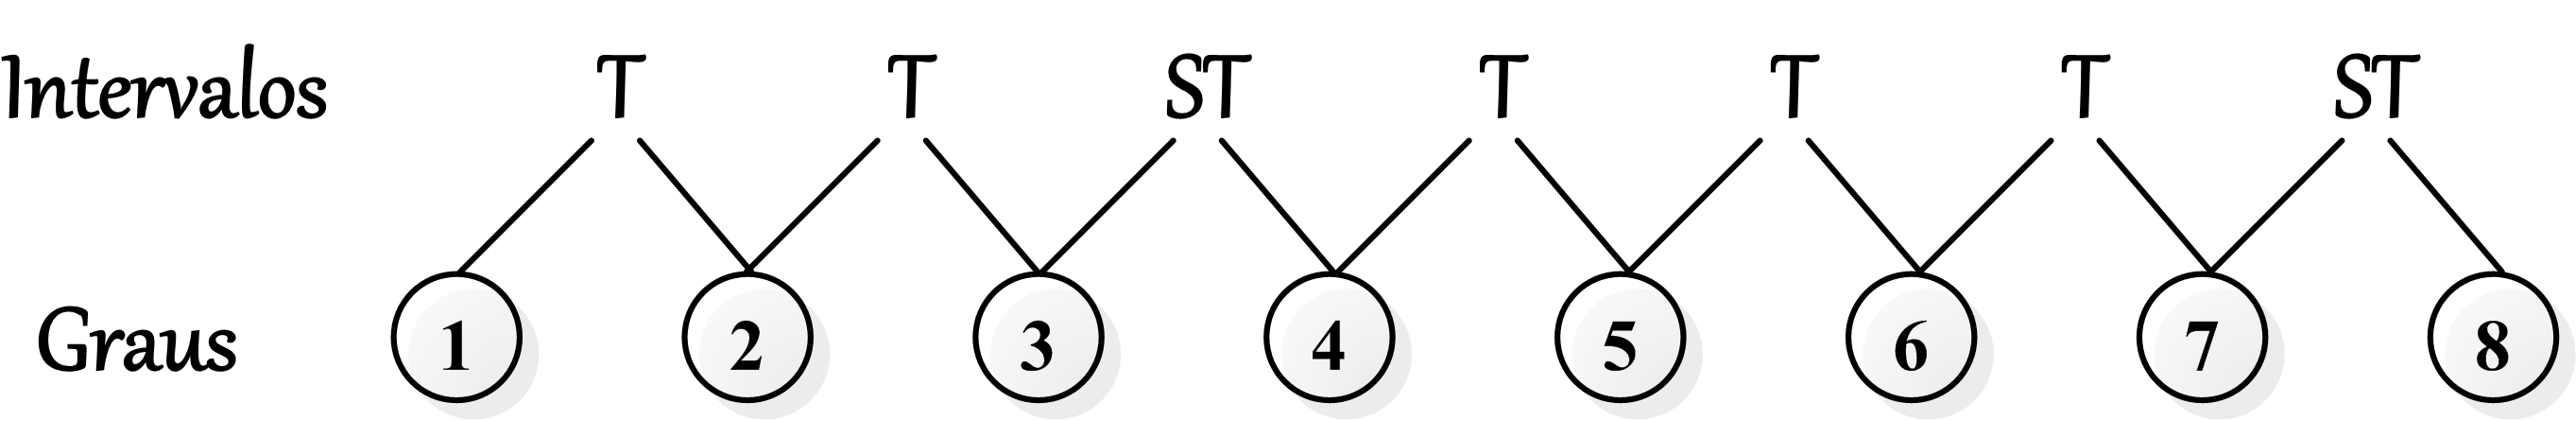
\includegraphics[scale=.9]{maior_natural.png}
      %\legend{Fonte: o autor}
    \end{center}
\end{figure}